%
%===============>>  ГРУППА 8-2 МОДУЛЬ 9  <<=============
%
\setmodule{9}

%BEGIN_FOLD % ====>>_____ Занятие 1 _____<<====
\begin{class}[number=1]
	\begin{listofex}
		\item В прямоугольный треугольник с катетами, равными \(6\) и 8, вписан квадрат, имеющий с треугольником общий прямой угол. Найдите сторону квадрата.
		\item Диагонали \(AC\) и \(BD \) выпуклого четырехугольника \(ABCD\), площадь которого равна \(28\), пересекаются в точке \(O\). Через середины отрезков \(BO\) и \(DO\) проведены прямые, параллельные диагонали \(AC\). Найдите площадь части четырехугольника, заключенной между этими прямыми.
		\item Основания \(AD\) и \(BC\) трапеции \(ABCD\) равны соответственно \(a\) и \(b\). Диагональ \(AC\) разделена на три равные части и через ближайшую к \(A\) точку деления \(M\) проведена прямая, параллельная основаниям. Найдите отрезок этой прямой, заключенный между диагоналями.
		\item Докажите, что медиана \(AM\) треугольника \(ABC\) делит пополам любой отрезок с концами на \(AB\) и \(AC\), параллельный стороне \(BC\). 
		\item Докажите, что точка пересечения диагоналей, точка пересечения продолжений боковых сторон и середины оснований любой трапеции лежат на одной прямой.
	\end{listofex}
\end{class}
%END_FOLD

%BEGIN_FOLD % ====>>_____ Занятие 2 _____<<====
\begin{class}[number=2]
	\begin{listofex}
		\item Докажите, что квадрат высоты прямоугольного треугольника, проведённой к гипотенузе, равен произведению проекций катетов на гипотенузу.
		\item Один из катетов прямоугольного треугольника равен \( 15 \), а проекция второго катета на гипотенузу равна \( 16 \). Найдите гипотенузу и второй катет.
		\item В треугольнике \( ABC \) с прямым углом \( C \) Проведена высота \( CD \). Известно, что на \( BC \) взята точка \( E \) и \( DE \) перпендикулярно \( BC \). Найдите \( DE \), если \( AC=15 \) см, а \( AD=9 \) см.	
		\item Медиана прямоугольного треугольника, проведенная к гипотенузе, равна \( 12 \) и делит прямой угол в отношении \( 1:2 \). Найдите стороны треугольника.
		\item Катеты прямоугольного треугольника равны \( 12 \) и \( 16 \). Найдите медиану, проведенную к гипотенузе.
		\item Найдите высоту трапеции со сторонами, равными \( 10 \), \( 10 \), \( 10 \) и \( 26 \).
		\item Найдите высоту равнобедренного треугольника, проведенную к основанию, если стороны треугольника равны \( 10 \), \( 13 \) и \( 13 \).
		\item Найдите высоту, а также радиусы вписанной и описанной окружностей равностороннего треугольника со стороной, равной \( a \).
		\item Вершина \( M \) правильного треугольника \( ABM \) со стороной \( a \) расположена на стороне \( CD \) прямоугольника \( ABCD \).	Найдите диагональ прямоугольника \( ABCD \).
	\end{listofex}
\end{class}
%END_FOLD

%BEGIN_FOLD % ====>>_ Домашняя работа 1 _<<====
\begin{homework}[number=1]
	\begin{listofex}
		\item Сторона \( AD \) параллелограмма \( ABCD \) разделена на \( n \) равных частей. Первая точка деления \( P \) соединена с вершиной \( B \). Докажите, что прямая \( BP \) отсекает на диагонали \( AC \) часть \( AQ \), которая равна \( \dfrac{1}{n+1} \)	всей диагонали.
		\item Точка \( M \) лежит на боковой стороне \( AC \) равнобедренного треугольника \( ABC \) с основанием \( BC \), причем \( BM=BC \). Найдите \( MC \), если \( BC=1 \) и \( AB=2 \).
		\item Найдите отношение оснований трапеции, если ее	средняя линия делится диагоналями на три равные части.
	\end{listofex}
\end{homework}
%END_FOLD

%BEGIN_FOLD % ====>>_____ Занятие 3 _____<<====
\begin{class}[number=3]
	\begin{listofex}
		\item Прямая, проведенная через вершину \( C \) трапеции \( ABCD \) параллельно диагонали \( BD \), пересекает продолжение основания \( AD \) в точке \( M \). Докажите, что треугольник \( ACM \) равновелик трапеции \( ABCD \).
		\item Проекция диагонали равнобокой трапеции на ее большее основание равна \( a \), боковая сторона равна \( b \). Найдите площадь трапеции, если угол при ее меньшем основании равен \( 150\degree \).
		\item Диагонали четырехугольника разбивают его на четыре треугольника. Известно, что треугольники, прилежащие к двум противоположным сторонам четырехугольника, равновелики. Докажите, что данный четырехугольник --- трапеция или параллелограмм.
		\item Точка внутри параллелограмма соединена со всеми его вершинами. Докажите, что суммы площадей треугольников, прилежащих к противоположным сторонам параллелограмма, равны между собой.
		\item Докажите, что если диагональ какого-нибудь четырехугольника делит другую диагональ пополам, то она разбивает этот четырехугольник на две равновеликие части.
		\item Середины сторон выпуклого четырехугольника последовательно соединены отрезками. Докажите, что площадь	полученного четырехугольника вдвое меньше площади исходного.
	\end{listofex}
\end{class}
%END_FOLD

%BEGIN_FOLD % ====>>_____ Занятие 4 _____<<====
\begin{class}[number=4]
	\begin{listofex}
		\item Основания равнобедренной трапеции равны \(8\) и \(18\), а периметр равен \(56\). Найдите площадь трапеции.
		\item Периметр прямоугольника равен \(56\), а диагональ равна \(27\). Найдите площадь этого прямоугольника.
		\item Прямая, параллельная основаниям \(MP\) и \(NK\) трапеции \(MNKP\), проходит через точку пересечения диагоналей трапеции и пересекает её боковые стороны \(MN\) и \(KP\) в точках  \(A\) и \(B\) соответственно. Найдите длину отрезка \(AB\), если \(MP=40\) см, \(NK=24\) см.
		\item В трапеции \(ABCD\) основание \(AD\) вдвое больше основания \(BC\) и вдвое больше боковой стороны \(CD\). Угол \(ADC\) равен \(60\degree\), сторона \(AB\) равна \(2\). Найдите площадь трапеции.
		\item В трапеции \(ABCD\) боковые стороны \(AB\) и \(CD\) равны, \(CH\) ---высота, проведённая к большему основанию \(AD\). Найдите длину отрезка \(HD\), если средняя линия \(KM\) трапеции равна \(16\), а меньшее основание \(BC\) равно \(4\).
		\item Основания трапеции равны \(16\) и \(34\). Найдите отрезок, соединяющий середины диагоналей трапеции.
		\item Найдите боковую сторону \(AB\) трапеции \(ABCD\), если углы \(ABC\) и \(BCD\) равны соответственно \(60\degree\) и \(150\degree\), а \(CD=33\).
	\end{listofex}
\end{class}
%END_FOLD

%BEGIN_FOLD % ====>>_ Домашняя работа 2 _<<====
\begin{homework}[number=2]
	\begin{listofex}
		\item В трапеции \(ABCD\) основание \(AD\) вдвое больше основания \(BC\) и вдвое больше боковой стороны \(CD\). Угол \(ADC\) равен \(60\degree\), сторона \(AB\) равна \(2\). Найдите площадь трапеции.
		\item В трапеции \(ABCD\) боковые стороны \(AB\) и \(CD\) равны, \(CH\) ---высота, проведённая к большему основанию \(AD\). Найдите длину отрезка \(HD\), если средняя линия \(KM\) трапеции равна \(16\), а меньшее основание \(BC\) равно \(4\).
		\item Периметр прямоугольника равен \( 30 \), а диагональ равна \( 14 \). Найдите площадь этого прямоугольника.
	\end{listofex}
\end{homework}
%END_FOLD

%BEGIN_FOLD % ====>>_____ Занятие 5 _____<<====
\begin{class}[number=5]
	\begin{listofex}
		\item Высоты \( AA_1 \) и \( BB_1 \) остроугольного треугольника \( ABC \) пересекаются в точке \( E \). Докажите, что	углы \( AA_1B_1 \) и \( ABB_1 \) равны.
		\item В равностороннем треугольнике \( ABC \) точки \( M \), \( N \), \( K \) --- середины сторон \( AB \), \( BC \), \( CA \) соответственно. Докажите, что треугольник \( MNK \) --- равносторонний.
		\item На стороне \( AC \) треугольника \( ABC \) отмечены точки \( D \) и \( E \) так, что \( AD=CE \). Докажите, что если \( BD=DE \), то \( AB=BC \).
		\item На медиане \( KF \) треугольника \( MKP \) отмечена точка \( E \). Докажите, что если \( EM=EP \), то \( KM=KP \).
		\item 
		\begin{minipage}[t]{\bodywidth}
			Два равносторонних треугольника имеют общую	вершину. Докажите, что отмеченные на рисунке отрезки \( AB \) и \( CD \) равны.
		\end{minipage}
		\gapwidth
		\begin{minipage}[t]{\picwidth}
			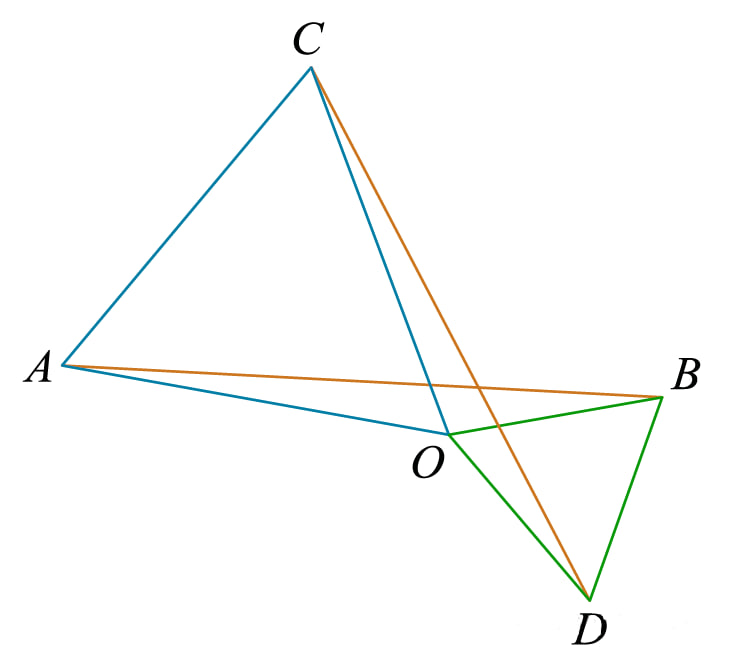
\includegraphics[align=t, width=\linewidth]{\picpath/G82M9L5}
		\end{minipage}
		\item Докажите, что у равных треугольников \( ABC \) и \( A_1B_1C_1 \) биссектрисы, проведённые из вершины \( A \) и \( A_1 \) равны.
	\end{listofex}
\end{class}
%END_FOLD

%BEGIN_FOLD % ====>>_____ Занятие 6 _____<<====
\begin{class}[number=6]
	\begin{listofex}
		\item Окружность касается всех сторон трапеции. Докажите, что боковая сторона трапеции видна из центра окружности под прямым углом.
		\item Диагонали равнобокой трапеции взаимно перпендикулярны. Докажите, что средняя линия трапеции равна высоте.
		\item \( AA_1 \) и \( BB_1 \) --- высоты остроугольного треугольника \( ABC \). Докажите, что треугольник \( AA_1C \) подобен треугольнику \( BB_1C \), а треугольник \( ABC \) подобен треугольнику \( A_1B_1C \).
		\item Пусть \( M \) и \( N \) --- проекции вершины \( A \) параллелограмма \( ABCD \) на прямые \( BC \) и \( CD \) соответственно. Докажите, что треугольник \( MAN \) подобен треугольнику \( ABC \).
		\item Через середину \( M \) стороны \( BC \) параллелограмма \( ABCD \), площадь которого равна \( 1 \), и вершину \( A \) проведена прямая, пересекающая диагональ \( BD \) в точке \( O \). Найдите площадь четырехугольника \( OMCD \).
		%\item На сторонах \( AB \) и \( AD \) параллелограмма \( ABCD \) взяты точки \( M \) и \( N \) так, что прямые \( MC \) и \( NC \) делят параллелограмм на три равновеликие части. Найдите \( MN \), если \( BD=d \).
		%\item Площади треугольников, образованных отрезками	диагоналей трапеции и ее основаниями, равны \( S_1 \) и \( S_2 \). Найдите	площадь трапеции.
	\end{listofex}
\end{class}
%END_FOLD

%BEGIN_FOLD % ====>>_ Домашняя работа 3 _<<====
\begin{homework}[number=3]
	\begin{listofex}
		\item Окружность касается всех сторон равнобокой трапеции. Докажите, что боковая сторона трапеции равна средней линии.
		\item Дана трапеция \( ABCD \) с основанием \( AD \). Биссектрисы внешних углов при вершинах \( A \) и \( B \) пересекаются в точке \( P \), а при вершинах \( C \) и \( D \) --- в точке \( Q \). Докажите, что отрезок \( PQ \) равен полупериметру трапеции.
		\item Основание треугольника равно \( 36 \). Прямая, параллельная основанию, делит треугольник на две равновеликие части. Найдите длину отрезка этой прямой, заключённого между сторонами треугольника.
	\end{listofex}
\end{homework}
%END_FOLD

%BEGIN_FOLD % ====>>_____ Занятие 7 _____<<====
\begin{class}[number=7]
	\begin{listofex}
		\item Докажите, что высота, проведённая из прямого угла прямоугольного треугольника, разделяет треугольник на два подобных прямоугольных треугольника, каждый из которых подобен данному треугольнику.
		\item В прямоугольном треугольнике \( ABC \) \( \angle C=90\degree \), \( СH \) --- высота, равная \( 4 \). Найдите \( AC \), \( BC \), \( HB \) и \( AB \), если \( AH=6 \).
		\item В прямоугольном треугольнике \( NKM \) с прямым углом \( K \) проведена высота \( KF \). Найдите \( KN \), \( KM \) и \( KF \), если \( MN=50 \), а \( KN:KM=3:4 \).
		\item В параллелограмме \( ABCD \) \( BD\perp AB \). Найдите площадь параллелограмма, если \( BE \) --- высота, равная \( 6 \), а \( AE=3 \).
		\item В прямоугольной трапеции \( MNKP \) (\( \angle N=90\degree \)) меньшее основание \( NK=16 \), а боковая сторона \( NM=12 \). Диагональ \( MK \) образует с другой боковой стороной угол \( 90\degree \). Найдите площадь трапеции.
		\item Найдите неизвестные элементы треугольника \( KNM \), угол \( K \) --- прямой:
		\begin{center}
			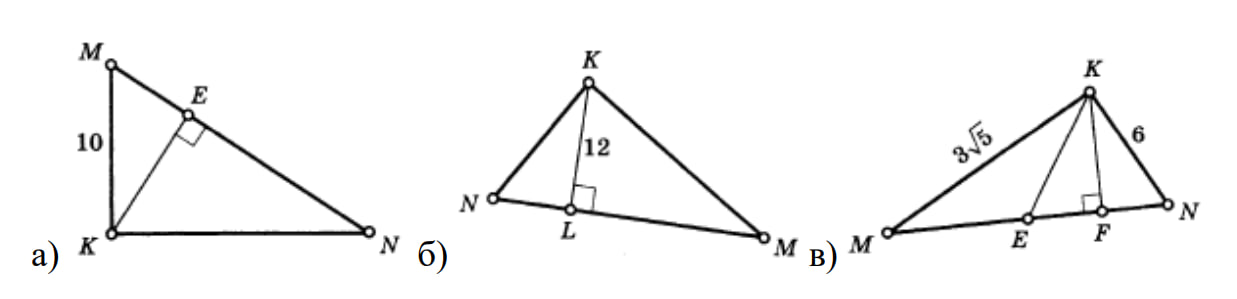
\includegraphics[align=t, width=0.9\linewidth]{\picpath/G82M9L7}
		\end{center}
	\end{listofex}
\end{class}
%END_FOLD

%BEGIN_FOLD % ====>>_ Проверочная работа _<<====
\begin{class}[number=8]
	\begin{listofex}
		\item Докажите, что биссектрисы углов при боковой стороне трапеции пересекаются на ее средней линии.
		\item На прямую, проходящую через вершину \( A \) треугольника \( ABC \), опущены перпендикуляры \( BD \) и \( CE \). Докажите, что середина стороны \( BC \) равноудалена от точек \( D \) и \( E \).
		\item Средняя линия трапеции равна \( 5 \), а отрезок, соединяющий середины оснований, равен \( 3 \). Углы при большем основании трапеции равны \( 30\degree \) и \( 60\degree \). Найдите основания и меньшую боковую сторону трапеции.
		\item Окружность, построенная на большем основании трапеции как на диаметре, проходит через середины боковых сторон и касается меньшего основания. Найдите углы трапеции.
		\item Одна из боковых сторон трапеции равна сумме оснований. Докажите, что биссектрисы углов при этой стороне пересекаются на другой боковой стороне.
	\end{listofex}
\end{class}
%END_FOLD